\documentclass[titlepage,a4paper]{article}

\usepackage{a4wide}
\usepackage[colorlinks=true,linkcolor=black,urlcolor=blue,bookmarksopen=true]{hyperref}
\usepackage{bookmark}
\usepackage{fancyhdr}
\usepackage[spanish]{babel}
\usepackage[utf8]{inputenc}
\usepackage[T1]{fontenc}
\usepackage{graphicx}
\usepackage{float}

\pagestyle{fancy} % Encabezado y pie de página
\fancyhf{}
\fancyhead[L]{TP1S - Max Mustermann}
\fancyhead[R]{Algoritmos y Programación III - FIUBA}
\renewcommand{\headrulewidth}{0.4pt}
\fancyfoot[C]{\thepage}
\renewcommand{\footrulewidth}{0.4pt}

\begin{document}
\begin{titlepage} % Carátula
	\hfill
\includegraphics[width=6cm]{logofiuba.jpg}
    \centering
    \vfill
    \Huge \textbf{Trabajo Práctico 1 — Smalltalk}
    \vskip2cm
    \Large [7507/9502] Algoritmos y Programación III\\
    Curso X \\ % Curso 1 para el de la tarde y 2 para el de la noche
    Primer cuatrimestre de 2018 
    \vfill
    \begin{tabular}{ | l | l | } % Datos del alumno
      \hline
      Alumno: & MUSTERMANN, Max \\ \hline
      Número de padrón: & 123456 \\ \hline
      Email: & mmustermann@fi.uba.ar \\ \hline
  	\end{tabular}
    \vfill
    \vfill
\end{titlepage}

\tableofcontents % Índice general
\newpage

\section{Introducción}\label{sec:intro}
El presente informe reune la documentación de la solución del primer trabajo práctico de la materia Algoritmos y Programación III que consiste en desarrollar una aplicación de un sistema de una agencia de viajes en Pharo utilizando los conceptos del paradigma de la orientación a objetos vistos hasta ahora en el curso.

\section{Supuestos}\label{sec:supuestos}
\textit{Deberá contener explicaciones de cada uno de los supuestos que el alumno haya tenido que adoptar a partir de situaciones que no estén contempladas en la especificación.}
\newline
\newline
\centerline{\textbf{[Reemplazar este texto con su producción]}}

\section{Detalles de implementación}\label{sec:implementacion}
% Explicaciones sobre la implementación interna de algunas clases que consideren que puedan llegar a resultar interesantes.

\subsection{Pilares del paradigma}
\textit{Explicar que pilares del paradigma utilizó para modelar sus clases; describiendo ventajas, desventajas (de los pilares) y las clases donde lo aplicó. No explique los pilares, sino la manera en que los utilizó.}
\newline
\newline
\centerline{\textbf{[Reemplazar este texto con su producción]}}
\newline
\newline
Sed lorem diam, imperdiet in suscipit sed, lacinia id est. 

\begin{verbatim}
| rango |
rango := (2 to: 20) asOrderedCollection.
Transcript show: rango ; cr.
rango copy do: [ :unNumero | unNumero isPrime ifFalse: [ rango remove: unNumero ] ].
Transcript show: rango.
\end{verbatim}

\subsection{Herencia o delegación}
\textit{Explicar porque utilizó herencia o delegación; describiendo ventajas, desventajas y las clases donde las aplicó. No explique los pilares, sino la manera en que los utilizó.}
\newline
\newline
\centerline{\textbf{[Reemplazar este texto con su producción]}}
\newline
\newline
Quisque tempus, tortor et convallis interdum, ipsum leo tempus ipsum, in molestie tortor arcu sit amet tellus. Praesent fermentum hendrerit nulla. In maximus ornare maximus. Nullam consectetur placerat enim sit amet lacinia. Etiam pellentesque tellus consectetur hendrerit iaculis. Sed non laoreet felis.

\section{Diagramas de clase}\label{sec:diagramasdeclase}
\textit{ Uno o varios diagramas de clases mostrando las relaciones estáticas entre las clases.  Puede agregarse todo el texto necesario para aclarar y explicar su diseño. Recuerden que la idea de todo el documento es que quede documentado y entendible cómo está implementada la solución. Todos los diagramas tienen que estar embebidos como imágenes en el informe de manera tal que entren en el ancho de una hoja A4 sin tener que rotarla. No se aceptarán diagramas en archivos sueltos.}
\newline
\newline
\centerline{\textbf{[Reemplazar este texto con su producción]}}
\newline
\newline
Nunc molestie facilisis diam in auctor. Nulla sed porta nibh, eu elementum erat. 

\begin{figure}[H]
\centering
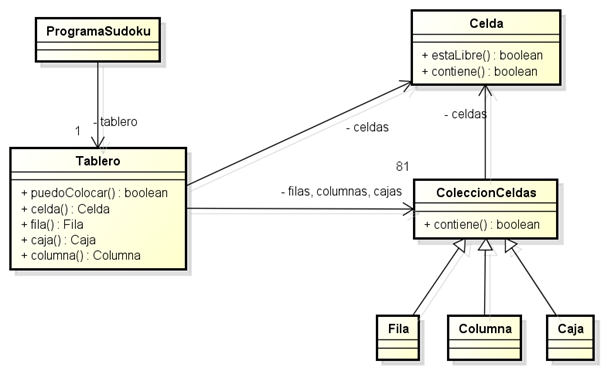
\includegraphics[width=0.8\textwidth]{diagrama_clase01.png}
\caption{\label{fig:class01}Diagrama del Sudoku.}
\end{figure}

\section{Diagramas de secuencia}\label{sec:diagramasdesecuencia}
\textit{Mostrar las secuencias interesantes que hayan implementado. Utilice su critério para elegir cual y el nivel de detalle a mostrar.}
\newline
\newline
\centerline{\textbf{[Reemplazar este texto con su producción]}}
\newline
\newline
Sed scelerisque est at augue finibus, at faucibus erat venenatis. 

\begin{figure}[H]
\centering
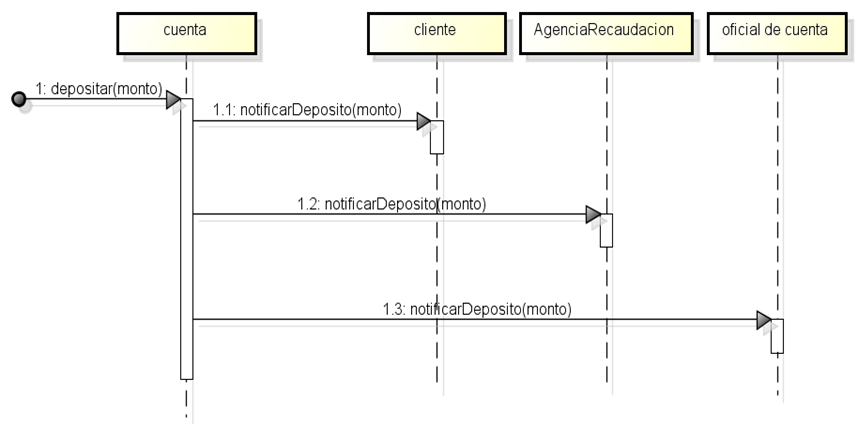
\includegraphics[width=0.8\textwidth]{diagrama_secuencia01.png}
\caption{\label{fig:seq01}Aliquam rutrum justo sed.}
\end{figure}

Cras est velit, aliquet quis sagittis ornare, volutpat ac risus. Sed ullamcorper tellus orci, non viverra nulla rhoncus nec. Vivamus pretium dui pellentesque dolor molestie facilisis. Pellentesque tristique egestas magna quis tincidunt. Suspendisse non urna dolor. Fusce arcu erat, posuere in nibh at, gravida vulputate ligula. Ut erat erat, facilisis ac tristique eget, mattis sit amet nulla.


\begin{figure}[H]
\centering
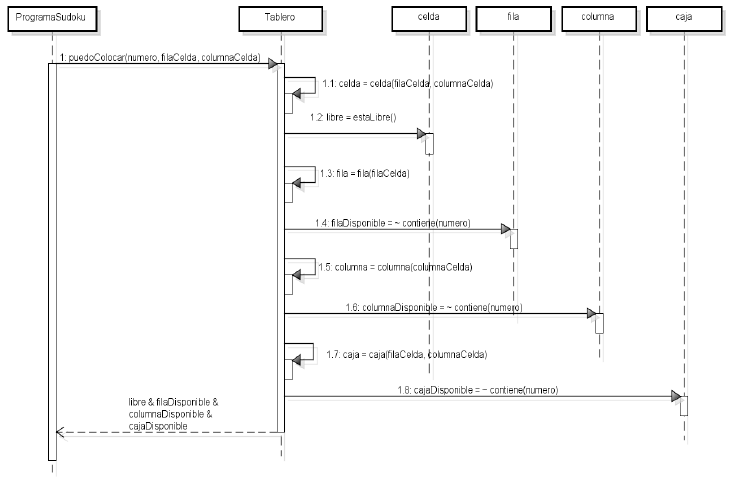
\includegraphics[width=\textwidth]{diagrama_secuencia02.png}
\caption{\label{fig:seq02}Nam a nulla non mauris ullamcorper.}
\end{figure}

Donec efficitur, sapien quis consectetur bibendum, metus magna finibus metus, id venenatis dolor est eu tortor. 

Sed sed diam in elit vulputate ultricies. Sed at felis mauris.


\section{Excepciones}\label{sec:excepciones}
\textit{ Explicación de cada una de las excepciones creadas y con qué fin fueron creadas (de manera concisa).}
\begin{description}
\item[Excepcion 1] \textbf{[Reemplazar este texto con su producción]}
\item[Excepcion n] \textbf{[Reemplazar este texto con su producción]}
\end{description}

\end{document}
